% Indicate the main file. Must go at the beginning of the file.
% !TEX root = ../main.tex

%%%%%%%%%%%%%%%%%%%%%%%%%%%%%%%%%%%%%%%%%%%%%%%%%%%%%%%%%%%%%%%%%%%%%%%%%%%%%%%%
% 04_discussion
%%%%%%%%%%%%%%%%%%%%%%%%%%%%%%%%%%%%%%%%%%%%%%%%%%%%%%%%%%%%%%%%%%%%%%%%%%%%%%%%


\section{Discussion}
\label{discussion}

\subsection{Detection}
The detection process significantly influenced the dataset composition, particularly on the sequence level for the category \textit{mustela\_erminea}.
This category experienced higher data loss, likely due to the relative size of the species --- it is much larger than the other species captured by these MammaliaBox camera traps.
This larger size may have resulted in more frequent bad shots due to the closeness to the camera or the speed at which they pass through the box --- many images showed only the tip of the animal's tail disappearing out of the box.
Another interesting observation was the fact that the white fur individuals were more often not detected than the brown fur individuals.
An explanation has yet to be found for why this was only the case on the sequence level, where the \textit{mustela\_erminea} category was disproportionately affected.
On the image level, the \textit{soricidae} category was the most affected, with \(23\%\) of the images lost but only \(1\%\) of the sequences.

Visual inspection revealed a mixture of exemplary BBox detections alongside notable inaccuracies, such as missed detections in images with obstructions or partial visibility of animals.
Looking through misclassified images with high confidence values revealed some interesting insights.
One was that quite a few false positive detections were made, leading to surprisingly high confidence classifications.
Some of these images were empty or contained no animal at all, as shown in \autoref{fig:false_positive_dt}, which includes examples where plant parts were misdetected, or possibly animals appeared in very dark areas, or some very small, not clearly visible objects.
Another interesting finding was that quite a few of the images contained a snail in the highest confidence BBox --- refer to \autoref{fig:false_class_snails} for a hand-picked selection of these examples.
These misclassifications highlight the need for enhanced object discrimination capabilities or the introduction of an additional class for non-target species.

The dilemma of not missing potentially relevant detections while also not polluting the dataset with image noise remains a challenge.
Simply to lower the detection threshold to reduce missed out animals is not a viable solution --- an improvement or the detection algorithm would be necessary to achieve this.

\begin{figure}[ht]
\centering
\includegraphics[width=\textwidth]{figures/false_positive_dt.pdf}
\caption{Hand-picked selection of images with a high confidence value but no animal in the image.}
\label{fig:false_positive_dt}
\end{figure}

\begin{figure}[ht]
\centering
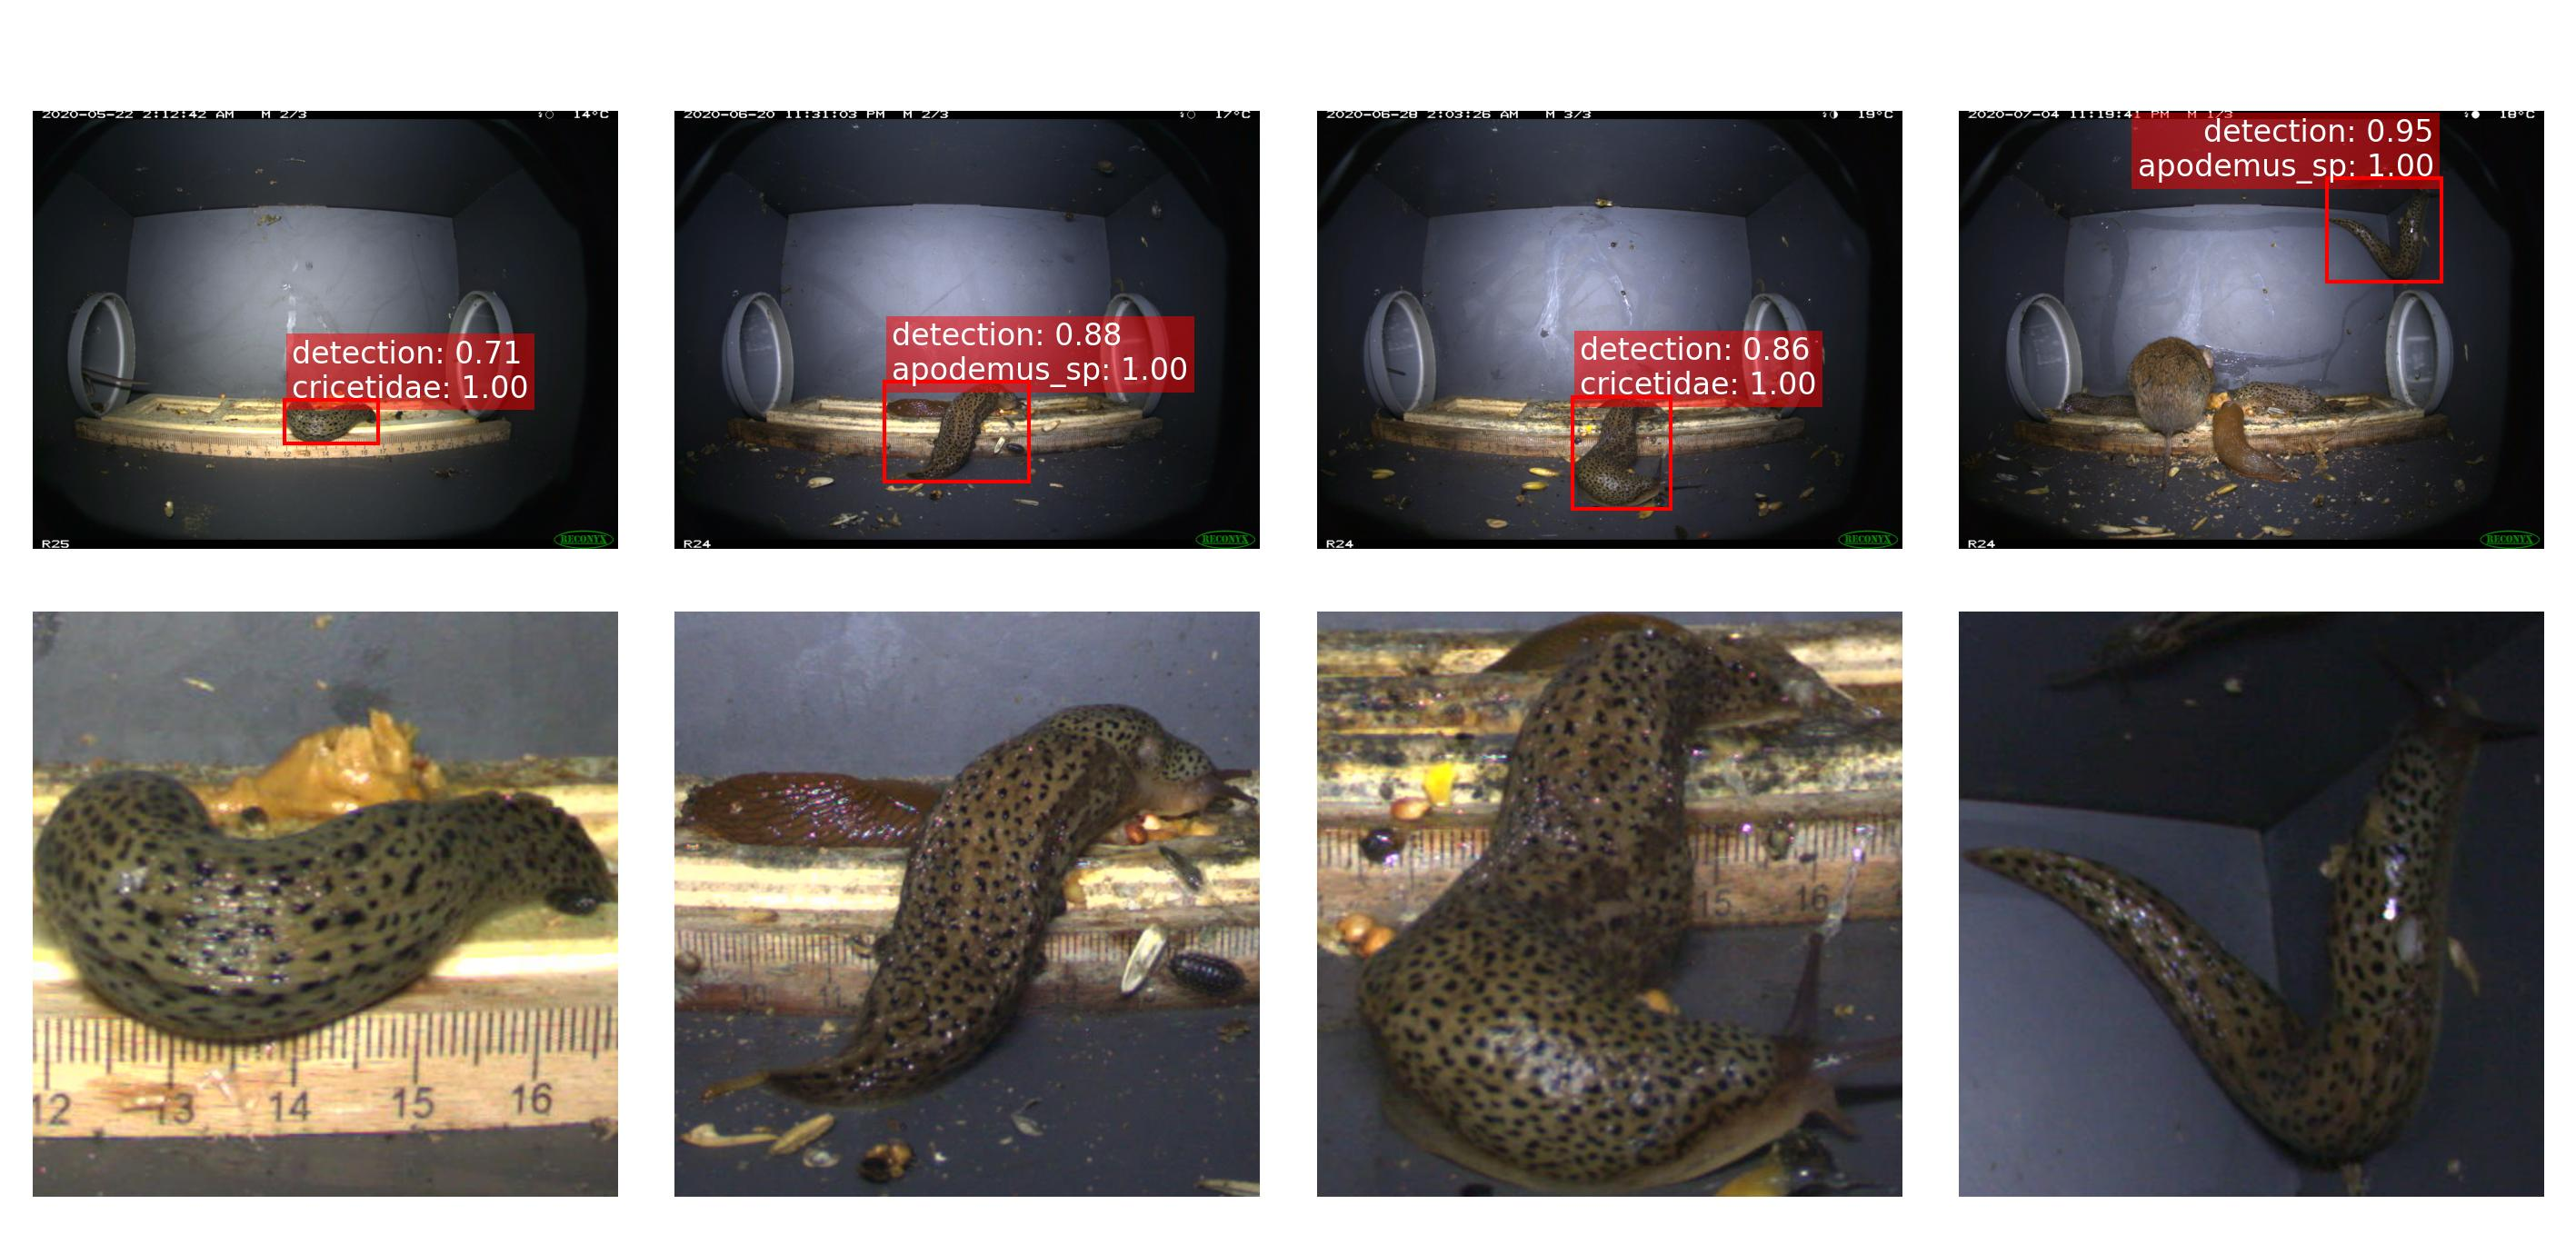
\includegraphics[width=\textwidth]{figures/false_class_snails.pdf}
\caption{Hand-picked selection of images predicted incorrectly with a high confidence value displaying a snail in the highest confidence BBox.}
\label{fig:false_class_snails}
\end{figure}

\subsection{Model Performance}
All tested models achieved high performance in image classification tasks, demonstrating their suitability for automating small mammal identification.
Pretrained models slightly outperformed those trained from scratch, underscoring the value of transfer learning.
The slightly better balanced accuracy of pretrained models is just one of the benefits of using pretrained models, as they also require less training time and computational resources and could potentially be trained with less training data.

Interestingly, the smaller the models, the better they performed on the image-level classification task, highlighting the fact that bigger is not always better.
Smaller models, if complex enough for the task, are always preferable since they require less computational resources and are faster to train.
Examining \autoref{fig:bal_acc_img} again, one could speculate about a trend for smaller models to perform more consistently across folds when trained from scratch --- but for some reason, this is not the case for the EfficientNet-B0 model.
The observations from this study suggest that smaller, computationally efficient models are sufficient and therefore preferable for the classification tasks at hand.

\subsection{Best Model Architecture}
The pretrained EfficientNet-B0 emerged as the best-performing architecture, achieving the highest \ac{BA}.
Remarkably, the optimal validation loss was reached within the first few epochs, while the accuracy continued to improve \autoref{fig:training_metrics_best_model}.\todo{Why did Accuracy still improve?}
Since the training dataset was quite large, contained only four classes, and was intensively vetted using the \ac{MD}, the model was able to learn the task quite quickly.
The initial supposition that a higher confidence in the detection would lead to a higher classification confidence could not be confirmed by the Spearman's rank corelation coefficient.
It even suggested that the correlation is stronger for the incorrect classifications.
Examining \autoref{fig:pred_conf_hexbin} of the relationship between detection confidence and classification confidence, shows that the classification confidence is generally very high --- for all detection confidence values and even for incorrect classifications.
There seems to be more values located in the upper right corner, which would point to a higher confidence detection leading to a higher classification confidence.
Since there is so many samples with close to 1 classification confidence trough all detection confidence values, the Spermann's rank might not be a good measure for this relationship.
This many very high classification confidence values could be explained considering the model's architecture.
In the last layers of the model, the following happens: the model maps its learned features to the four classes and than normalizes this for values to sum to one.
If the model is entirely confident that an input does not belong to the first three classes and assigns a very small value to the fourth class (e.g., $[0\;;\;0\;;\;0\;;\;10^{-5}]$), this distribution will be normalized to $[0\;;\;0\;;\;0\;;\;1]$, resulting in a prediction for the fourth class with maximum confidence.
Therefore this evaluation lacks some meaningfulness.
It could be repeated with a predicted test set where the values are kept as they are without normalization.
Still, the assumption that a non-target class would benefit the classification task remains valid.

\begin{figure}[ht]
\centering
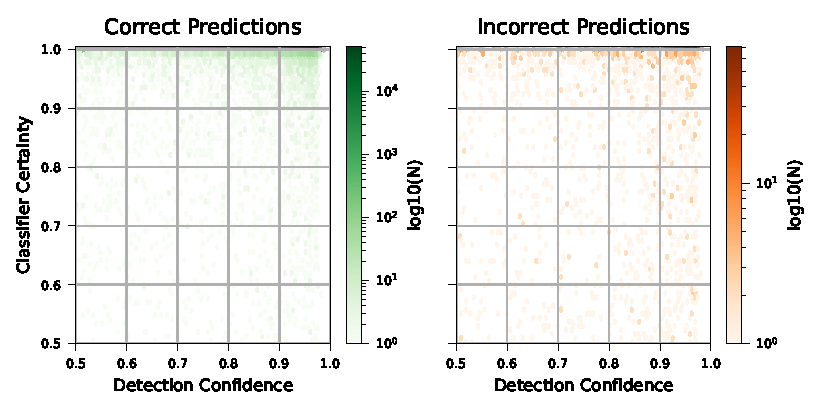
\includegraphics{figures/pred_conf_hexbin.pdf}
\caption{Hexbin plot of detection confidence vs. classifier confidence for correct and incorrect classifications. Color scale indicates log$_{10}$-binned counts.}
\label{fig:pred_conf_hexbin}
\end{figure}

\subsection{Limitations}\todo{this is not ready}
The primary limitation of the current methodology is the absence of an explicit non-target class, forcing models into potentially incorrect predictions, exemplified by the snail misclassification issue, shown in \autoref{fig:false_class_snails}.
Further, despite improvements, the \ac{MD} still misses a significant number of potentially relevant detections.
This limitation is particularly pronounced for rare species, where insufficient data reduces detection reliability.
The loss of sequences for the \textit{mustela\_erminea} category, as shown in \autoref{tab:data_availability_after_md}, illustrates this issue.
Every sequence completely lost is a potentially missed sighting of a rare species, which could have provided valuable insights for conservation efforts.

The step of the sequence classification is performed on the model's outputted classification confidence values per class and image.
Since the information from the output on the logits level is heavily distorted by the normalization step, the sequence classification is not yet to its full potential.
This approach might need to be revisited in order to improve the reliability of the sequence classification results.

Moreover, the current approach is heavily dependent on data availability.
Rare species inherently have fewer data points, constraining model training and potentially biasing predictions.
To include an additional class would require a sufficient number of samples to ensure reliable model performance and generally, the data acquisition is the moste resource intensive part of most machine learning projects.
